% Options for packages loaded elsewhere
\PassOptionsToPackage{unicode}{hyperref}
\PassOptionsToPackage{hyphens}{url}
\documentclass[
  11pt,
  a4paper,
]{article}
\usepackage{xcolor}
\usepackage[margin=22mm]{geometry}
\usepackage{amsmath,amssymb}
\setcounter{secnumdepth}{-\maxdimen} % remove section numbering
\usepackage{iftex}
\ifPDFTeX
  \usepackage[T1]{fontenc}
  \usepackage[utf8]{inputenc}
  \usepackage{textcomp} % provide euro and other symbols
\else % if luatex or xetex
  \usepackage{unicode-math} % this also loads fontspec
  \defaultfontfeatures{Scale=MatchLowercase}
  \defaultfontfeatures[\rmfamily]{Ligatures=TeX,Scale=1}
\fi
\usepackage{lmodern}
\ifPDFTeX\else
  % xetex/luatex font selection
\fi
% Use upquote if available, for straight quotes in verbatim environments
\IfFileExists{upquote.sty}{\usepackage{upquote}}{}
\IfFileExists{microtype.sty}{% use microtype if available
  \usepackage[]{microtype}
  \UseMicrotypeSet[protrusion]{basicmath} % disable protrusion for tt fonts
}{}
\makeatletter
\@ifundefined{KOMAClassName}{% if non-KOMA class
  \IfFileExists{parskip.sty}{%
    \usepackage{parskip}
  }{% else
    \setlength{\parindent}{0pt}
    \setlength{\parskip}{6pt plus 2pt minus 1pt}}
}{% if KOMA class
  \KOMAoptions{parskip=half}}
\makeatother
\usepackage{longtable,booktabs,array}
\newcounter{none} % for unnumbered tables
\usepackage{calc} % for calculating minipage widths
% Correct order of tables after \paragraph or \subparagraph
\usepackage{etoolbox}
\makeatletter
\patchcmd\longtable{\par}{\if@noskipsec\mbox{}\fi\par}{}{}
\makeatother
% Allow footnotes in longtable head/foot
\IfFileExists{footnotehyper.sty}{\usepackage{footnotehyper}}{\usepackage{footnote}}
\makesavenoteenv{longtable}
\usepackage{graphicx}
\makeatletter
\newsavebox\pandoc@box
\newcommand*\pandocbounded[1]{% scales image to fit in text height/width
  \sbox\pandoc@box{#1}%
  \Gscale@div\@tempa{\textheight}{\dimexpr\ht\pandoc@box+\dp\pandoc@box\relax}%
  \Gscale@div\@tempb{\linewidth}{\wd\pandoc@box}%
  \ifdim\@tempb\p@<\@tempa\p@\let\@tempa\@tempb\fi% select the smaller of both
  \ifdim\@tempa\p@<\p@\scalebox{\@tempa}{\usebox\pandoc@box}%
  \else\usebox{\pandoc@box}%
  \fi%
}
% Set default figure placement to htbp
\def\fps@figure{htbp}
\makeatother
\setlength{\emergencystretch}{3em} % prevent overfull lines
\providecommand{\tightlist}{%
  \setlength{\itemsep}{0pt}\setlength{\parskip}{0pt}}
\usepackage{bookmark}
\IfFileExists{xurl.sty}{\usepackage{xurl}}{} % add URL line breaks if available
\urlstyle{same}
\hypersetup{
  pdftitle={Thue equations{,} effectively},
  pdfauthor={GPT-6 Astra (OpenAI), Ultra},
  hidelinks,
  pdfcreator={LaTeX via pandoc}}

\title{Thue equations, effectively}
\author{GPT-6 Astra (OpenAI), Ultra}
\date{October 2026}

\providecommand{\Eta}{\mathrm{H}}
\begin{document}
\maketitle

\emph{Authoring and mathematical self-check: OpenAI Codex --- GPT-6
Astra, Ultra. Original exposition, CC0.}

A product equation gives control of norms, whereas a logarithmic
estimate needs control of heights. Units can move the archimedean sizes
of an algebraic integer without changing its norm. We first make that
adjustment explicit, then apply the effective unit equation to a
relation among three factors.

The balancing idea occurs in the free paper of
\href{https://matwbn.icm.edu.pl/ksiazki/aa/aa74/aa7416.pdf}{Bugeaud and
Győry, \emph{Bounds for the solutions of unit equations}, Lemma 2}. The
proof below uses the complete quantitative fundamental-system and
unit-equation proofs of Lesson 12. Its constants are intentionally
large; their linear dependence on the height of the varying right-hand
side is the essential feature.

\subsection{Prerequisite proofs}\label{prerequisite-proofs}

{\def\LTcaptype{none} % do not increment counter
\begin{longtable}[]{@{}
  >{\raggedright\arraybackslash}p{(\linewidth - 2\tabcolsep) * \real{0.5000}}
  >{\raggedright\arraybackslash}p{(\linewidth - 2\tabcolsep) * \real{0.5000}}@{}}
\toprule\noalign{}
\begin{minipage}[b]{\linewidth}\raggedright
Input
\end{minipage} & \begin{minipage}[b]{\linewidth}\raggedright
Programme proof
\end{minipage} \\
\midrule\noalign{}
\endhead
\bottomrule\noalign{}
\endlastfoot
Heights, conjugates, the product formula and effective Northcott
finiteness & \href{../TR-TRANS/TR-TRANS-02.html}{Heights of algebraic
numbers, Theorems 2.4 and 2.6--2.8, Proposition 2.5} \\
Dirichlet units and the logarithm lattice &
\href{../NT-ANT/dirichlets-unit-theorem.html\#producing-enough-units}{Number
fields, Dirichlet's unit theorem, Theorem 9.2} \\
Discriminant and lattice index &
\href{../NT-ANT/discriminants-and-integral-bases.html}{Number fields,
Discriminants and integral bases, Proposition 2.2} \\
General and refined two-logarithm estimates &
\href{TR-BAKER-07.html\#1-an-explicit-bound-without-multiplicative-independence}{Lesson
7, Theorem 7.1},
\href{TR-BAKER-07.html\#11-a-sharper-bound-when-the-real-bases-are-close-to-one}{Theorem
7.6} and
\href{TR-BAKER-07.html\#12-a-rational-number-close-to-one}{Corollary
7.7} \\
Quantitative fundamental units and the effective unit equation &
\href{TR-BAKER-12.html\#4-effective-control-of-a-fundamental-system}{Lesson
12, Lemma 12.5} and
\href{TR-BAKER-12.html\#5-the-effective-unit-equation}{Theorem
12.6} \\
Roth's theorem and the limitation of its effectivity &
\href{../TR-TRANS/TR-TRANS-12.html\#theorem-12-1-roth-s-theorem}{Rational
approximation III, Theorem 12.1} and
\href{../TR-TRANS/TR-TRANS-12.html\#4-why-the-proof-gives-finiteness-without-a-denominator-bound}{Section
4} \\
\end{longtable}
}

\subsection{1. Representatives of principal ideals with controlled
height}\label{representatives-of-principal-ideals-with-controlled-height}

Let \(L\) be a number field of degree \(D\), absolute discriminant
\(\Delta_L\), and unit rank \(r\). Choose the fundamental units of Lemma
12.5, so \(h(\varepsilon_i)\le V=V(D,\Delta_L)\). At an infinite place
put \(n_v=1\) or \(2\), and use \(\lambda(z)_v=n_v\log|\sigma_vz|\).

\textbf{Lemma 13.1 (balancing by a unit).} If \(z\in O_L\setminus\{0\}\)
and \(k\ge1\) is an integer, there is a unit \(\epsilon\) such that \[
h(\epsilon^kz)\le
\frac{\log|N_{L/\mathbb Q}z|}{D}
+\frac{k}{2}\sum_{i=1}^r h(\varepsilon_i).
\tag{13.1}
\] One can effectively find a unit satisfying the slightly larger bound
\[
h(\epsilon^kz)\le
\frac{\log|N_{L/\mathbb Q}z|}{D}+krV.
\tag{13.2}
\] For \(r=0\) the empty sums are zero and \(\epsilon=1\) works.

\textbf{Proof.} Write \(M_z=|N_{L/\mathbb Q}z|\ge1\), and let
\(a_v=(n_v/D)\log M_z\). The vector \(\lambda(z)-a\) has coordinate sum
zero. Express it as \(\sum_i t_i\lambda(\varepsilon_i)\), using the
logarithm lattice basis from Dirichlet's theorem. Choose integers
\(b_i\) nearest to \(-t_i/k\) and put
\(\epsilon=\prod_i\varepsilon_i^{b_i}\). Then \[
\lambda(\epsilon^kz)=a+w,\qquad
w=k\sum_i c_i\lambda(\varepsilon_i),\qquad |c_i|\le\tfrac12,
\qquad \sum_vw_v=0.
\tag{13.3}
\] The element remains integral, so its height is the sum of the
positive infinite logarithms divided by \(D\). Since every \(a_v\) is
nonnegative, \[
\begin{aligned}
D h(\epsilon^kz)
&\le\log M_z+\sum_v\max(0,w_v)\\
&=\log M_z+\tfrac12\sum_v|w_v|\\
&\le\log M_z+kD\sum_i|c_i|h(\varepsilon_i).
\end{aligned}
\] This proves (13.1).

For effectivity when \(r\ge1\), enumerate integral-basis coordinate
boxes in \(O_L\) and retain the elements of absolute norm one; these are
exactly the units. Heights and \(\log M_z\) have arbitrarily accurate
rational interval approximations, obtained from isolated algebraic
conjugates and real logarithms. At stage \(j\), inspect the units in the
coordinate box of radius \(j\) with interval precision tending to
infinity, and stop when the strict inequality in (13.2) is certified.
The unit whose existence was proved in (13.1) satisfies that strict
inequality, because \(\sum_i h(\varepsilon_i)\le rV\) and \(krV>0\). It
eventually occurs in the search, and its positive margin is eventually
certified. Thus the search terminates, without requiring an algorithmic
choice of the short fundamental system. For \(r=0\), the logarithm
hyperplane is zero-dimensional, so \(\lambda(z)=a\) and \(\epsilon=1\)
works directly. \(\square\)

In particular the bound in Lemma 12.5 supplies a computable \(V\)
without a numerical decision about any exact logarithmic relation.

\subsection{2. A height bound for a general Thue
equation}\label{a-height-bound-for-a-general-thue-equation}

Fix a number field \(K\), and a homogeneous form \[
F(X,Y)=a\prod_{j=1}^n(X-\theta_jY)\in K[X,Y],
\qquad a\ne0,\qquad n\ge3,
\tag{13.4}
\] whose roots include at least three distinct elements. Renumber three
such roots as \(\theta_1,\theta_2,\theta_3\). Repeated additional roots
are allowed. Fix a splitting field \(L\supset K\), with degree \(D\),
discriminant \(\Delta_L\) and unit rank \(r\). All constants below
depend only on this fixed data. Choose integers \(M,P,U\ge1\) such that
\[
M\theta_j\in O_L,\qquad h(a)\le P,\qquad h(\theta_j)\le U
\quad(1\le j\le n).
\tag{13.5}
\] Such constants are effective from minimal polynomials and height
bounds. Put \(G=C_{\rm unit}(D,\Delta_L)\), as in (12.31), and use an
effective common unit-height bound \(V\) as above. Define \[
\begin{gathered}
T=1+nM+P+rV,\qquad W=4U+2+2T,\\
Z=2T+GW,\qquad B_0=3Z+2M+3U+3,\\
E=P+n(2B_0+U+1),\qquad C=1+E+nB_0.
\end{gathered}
\tag{13.6}
\]

\textbf{Theorem 13.2.} For every \(m\in K^\times\), every
\((x,y)\in O_K^2\) with \(F(x,y)=m\) satisfies \[
\max\{h(x),h(y)\}\le C\max\{h(m),1\}.
\tag{13.7}
\] In particular a finite search for all solutions can be bounded
effectively.

\textbf{Proof.} Set \(H=\max\{h(m),1\}\) and \(z_j=M(x-\theta_jy)\).
These are nonzero algebraic integers in \(L\), and \[
\prod_jz_j=M^nm/a.
\tag{13.8}
\] Each absolute norm \(|N z_j|\) is a positive integer. Their product
is \(|N(M^nm/a)|\); therefore \[
0\le\frac{\log|Nz_j|}{D}
\le h(m)+n\log M+h(a).
\tag{13.9}
\] The second inequality follows from \(\log|Nt|\le D h(t)\) and the
height product inequalities. It does not assume that \(m/a\) is integral
independently of the equation.

Apply (13.2) with \(k=1\), writing \(z_j=\gamma_j\eta_j\), where
\(\eta_j\) is a unit and \[
h(\gamma_j)\le TH.
\tag{13.10}
\] The identity \[
(\theta_1-\theta_2)z_3+
(\theta_2-\theta_3)z_1+
(\theta_3-\theta_1)z_2=0
\tag{13.11}
\] follows by substituting \(z_j=M(x-\theta_jy)\): the coefficients of
both \(x\) and \(y\) cancel. After division it becomes
\(\alpha u+\beta v=1\), where \[
\begin{gathered}
u=\eta_1/\eta_3,\quad v=\eta_2/\eta_3,\\
\alpha=\frac{(\theta_2-\theta_3)\gamma_1}
              {(\theta_2-\theta_1)\gamma_3},\qquad
\beta=\frac{(\theta_3-\theta_1)\gamma_2}
             {(\theta_2-\theta_1)\gamma_3}.
\end{gathered}
\tag{13.12}
\] All factors in the two coefficients are nonzero. Since
\(h(\theta_i-\theta_j)\le2U+\log2\), (13.10) gives
\(\max\{h(\alpha),h(\beta),1\}\le WH\). Theorem 12.6, applied in the
fixed field \(L\), yields \(h(u),h(v)\le GWH\). Consequently the two
ratios \[
\xi_1=z_1/z_3,\qquad \xi_2=z_2/z_3
\quad\hbox{satisfy}\quad h(\xi_i)\le ZH.
\tag{13.13}
\]

Recover the two original coordinates up to the remaining scale: \[
y=z_3 b,\quad x=z_3 c,\qquad
b=\frac{\xi_1-\xi_2}{M(\theta_2-\theta_1)},\quad
c=\frac{\xi_1}{M}+\theta_1b.
\tag{13.14}
\] These equalities follow by subtracting the first two factors. The
height inequalities, including \(h(0)=0\), give \[
h(b)\le(2Z+M+2U+2)H,\qquad h(c)\le B_0H.
\tag{13.15}
\] The first displayed constant is at most \(B_0\). Using the fixed
factorization (13.4), therefore, \[
h(F(c,b))\le
P+\sum_j\bigl(h(c)+h(\theta_j)+h(b)+\log2\bigr)
\le EH.
\tag{13.16}
\] Homogeneity now controls the scale: \(m=z_3^nF(c,b)\). Here
\(F(c,b)\ne0\), since \(m\ne0\). Thus \[
n h(z_3)\le h(m)+h(F(c,b))\le(1+E)H.
\tag{13.17}
\] Combining (13.14)--(13.17) bounds both coordinate heights by
\(((1+E)/n+B_0)H\), which is at most \(CH\). Northcott's explicit
coefficient-box proof then provides an effective finite list of possible
\(x,y\) in the fixed field; test integrality and the equation exactly.
This proves the height estimate and its effective finiteness
consequence. \(\square\)

\textbf{Corollary 13.3 (integer solutions).} For a fixed integral form
satisfying (13.4), there is an effective integer \(C_{\mathbb Z}\ge1\)
such that, for every nonzero integer \(m\), \[
F(x,y)=m,\quad x,y\in\mathbb Z
\quad\Longrightarrow\quad
\max\{|x|,|y|\}\le |2m|^{C_{\mathbb Z}}.
\tag{13.18}
\] One may take \(C_{\mathbb Z}=2C\).

\textbf{Proof.} For an integer \(x\), \(h(x)=\log\max\{1,|x|\}\). For
\(|m|\ge1\), \(\max\{\log|m|,1\}\le2\log(2|m|)\), because \(\log2>1/2\).
Exponentiate (13.7). \(\square\)

\subsection{3. An effective improvement of Liouville's
exponent}\label{an-effective-improvement-of-liouvilles-exponent}

\textbf{Theorem 13.4.} Let \(\theta\) be a real algebraic number of
degree \(n\ge3\). There are effective constants \(\tau(\theta)>0\) and
\(c(\theta)>0\) such that, for every integer \(p\) and every integer
\(q\ge1\), \[
|\theta-p/q|\ge c(\theta)q^{-n+\tau(\theta)}.
\tag{13.19}
\]

\textbf{Proof.} Homogenize the primitive minimal polynomial of
\(\theta\), obtaining an integral form
\(F(X,Y)=a\prod_{j=1}^n(X-\theta_jY)\). It is separable in
characteristic zero, so its roots are distinct. For any rational
\(p/q\), \(m=F(p,q)\) is a nonzero integer: zero would give a rational
root of an irreducible polynomial of degree at least three. Let
\(C_{\mathbb Z}\ge1\) be the constant in (13.18). It gives \[
|m|\ge\tfrac12 q^{1/C_{\mathbb Z}}.
\tag{13.20}
\] Choose an effective integer
\(A\ge\max\{1,|a|\prod_{j\ne1}(1+|\theta-\theta_j|)\}\). If
\(|p/q-\theta|\le1\), factorization gives \[
|m|\le A q^n|\theta-p/q|.
\tag{13.21}
\] Combining the two inequalities proves (13.19) with
\(\tau(\theta)=1/C_{\mathbb Z}\) and \(c(\theta)=1/(2A)\). If the error
exceeds one, the same conclusion holds because \(\tau\le1<n\), \(q\ge1\)
and \(c\le1\). All constants were determined from the minimal
polynomial; there is no unknown finite exceptional set. \(\square\)

This improves the Liouville exponent by a computable positive amount.
Roth gives the much stronger exponent \(2+\epsilon\) with finitely many
exceptions, but its programme proof does not compute the last exception.
Neither conclusion substitutes for the other.

\subsection{4. Bounding the exponent in a binomial
equation}\label{bounding-the-exponent-in-a-binomial-equation}

The exponent may itself be unknown. The important feature of the
two-logarithm estimate is its normalized coefficient \(B'\): after
division by a height, the remaining inequality involves \(n/H\).

\textbf{Theorem 13.5 (a uniform exponent bound).} Let \(a,b,c\) be
nonzero integers, let \(n\ge3\), and suppose \[
ax^n-by^n=c,\qquad x,y\in\mathbb Z,\qquad |xy|>1.
\tag{13.22}
\] With \[
H=\max\{1,\log|a|,\log|b|,\log|c|\},
\] one has the explicit bound \[
n<10^8H.
\tag{13.23}
\] No coprimality or multiplicative-independence assumption is required.

\textbf{Proof.} Put \(X=\max\{|x|,|y|\}\ge2\) and
\(Y=\min\{|x|,|y|\}\ge1\). Let \(A,B\) be the absolute values of the
coefficients attached to \(X,Y\), respectively, and set
\(P=AX^n,\ Q=BY^n\). If the original signed terms have opposite signs,
\(P+Q=|c|\), and \(n\log X\le\log|c|\le H\). This already gives
\(n<2H\).

Otherwise \(|P-Q|=|c|\). If \(|c|\ge P/2\), then \(X^n\le2|c|\), so \[
n\le\frac{H+\log2}{\log X}<3H.
\tag{13.24}
\] We can therefore assume \(0<|c|<P/2\). The real logarithmic form \[
\Gamma=\log(B/A)+n\log(Y/X)=\log(Q/P)
\tag{13.25}
\] is nonzero. Integrating \(1/(1+t)\) on the interval between zero and
\((Q-P)/P\), where \(|t|<1/2\), gives \[
0<|\Gamma|\le\frac{2|c|}{P}\le2|c|X^{-n}.
\tag{13.26}
\] Apply Theorem 7.1 with \(D=1\), height parameters
\(a_1=H,\ a_2=\max\{1,\log X\}\), and coefficients \(1,n\). For a
rational number \(u/v\), its height is the logarithm of the larger
absolute reduced numerator and denominator. Hence these parameters
dominate both rational heights and absolute real logarithms. The theorem
also covers a base equal to one and dependent bases, provided the
displayed form is nonzero.

Write \(t=n/H\). Since \(a_2\le(\log X)/\log2<2\log X\), its conclusion
gives \[
\log|\Gamma|\ge
-43200H\log X\,\max\{10,\log(t+1)\}^2.
\tag{13.27}
\] Indeed \(B'=1/a_2+n/H\le1+t\). Comparison with (13.26), and division
by \(H\log X\), yields \[
t\le3+43200\max\{10,\log(t+1)\}^2.
\tag{13.28}
\] For \(t\ge10^8\), the logarithm exceeds \(10\), and \[
\frac{3+43200\log^2(t+1)}{t}
\] is decreasing: its derivative has the sign of \[
-3+43200\log(t+1)
 \left(\frac{2t}{t+1}-\log(t+1)\right)<0.
\] At \(t=10^8\), use \(\log(10^8+1)<\log2+8\log10<21\). The numerator
is then less than \(3+43200\cdot21^2=19051203<10^8\), contradicting
(13.28). Here \(\log2<1,\ \log10<5/2\) follow, for example, from the
positive Taylor sums for \(e\) and \(e^{5/2}\). This proves (13.23).
\(\square\)

For fixed \(a,b,c\), Theorem 13.5 leaves a computable finite list of
exponents \(n\ge3\). For each exponent the polynomial \(aX^n-bY^n\) has
\(n\) distinct roots in characteristic zero. Corollary 13.3 then bounds
both coordinates. Thus the two results together give a terminating
enumeration of all solutions with \(|xy|>1\). Solutions with \(|xy|=1\)
must be considered separately: for instance \(a-b=c\) gives \(x=y=1\)
for every exponent.

\subsection{5. A family with a bound independent of its
coefficient}\label{a-family-with-a-bound-independent-of-its-coefficient}

For the adjacent-coefficient family a large radius in the two-logarithm
estimate removes the coefficient from the final bound. The following
proof uses Theorem 7.6 and Corollary 7.7, including the elementary
treatment of dependent rational bases.

\textbf{Theorem 13.6.} For every integer \(b\ge1\) and every integer
\(n\ge100000\), the equation \[
(b+1)x^n-by^n=1
\tag{13.29}
\] has exactly one solution in positive integers: \(x=y=1\).

\textbf{Proof.} Suppose a different positive solution exists. If
\(x\ge y\), then \((b+1)x^n-by^n\ge x^n\), forcing \(x=y=1\).
Consequently \(y>x\), and in fact \(y\ge b+2\). For if \(y\le b+1\),
then \(x/y\le(y-1)/y\le b/(b+1)\), whence \[
\frac{(b+1)x^n}{by^n}
\le\left(\frac b{b+1}\right)^{n-1}<1,
\] contrary to (13.29). Define \[
\delta=\frac1{by^n}
=\frac{b+1}{b}\left(\frac xy\right)^n-1>0.
\tag{13.30}
\]

First take \(b\ge5\). Apply Corollary 7.7 with
\((x_1,y_1,x_2,y_2)=(y,x,b+1,b)\). Its radius parameter satisfies \[
\eta=\frac{\log b}{\log(b+1)}>\frac45,\qquad
\eta\log(b+1)=\log b.
\] To verify the first inequality without a decimal approximation,
observe that \((1+1/b)^4\le(6/5)^4<5\le b\); therefore \((b+1)^4<b^5\).
All other hypotheses hold: \(y\ge7,\ y\ne x\), \((b+1)/b\le6/5\), and
the logarithmic form does not vanish because \(\delta>0\). Comparing
(7.33) with (13.30) gives \[
n<44\max\left\{1+\frac{\log n}{\log b},10\right\}^{2}
\le44\max\left\{1+\frac{\log n}{\log5},10\right\}^{2}.
\tag{13.31}
\] At \(n=100000\) the last maximum is \(10\): \(\log5>3/2\) and
\(\log100000<25/2\) suffice. Its right side is then \(4400<100000\). For
\(n\ge100000\), the quotient of that right side by \(n\) decreases. It
decreases on the constant branch; on the other branch the derivative has
the sign of \(2-(\log n+\log5)<0\). The two branches agree at their
junction. Thus (13.31) is impossible throughout the asserted range.

It remains to handle \(1\le b\le4\). The rational numbers
\(\alpha_1=y/x>1,\ \alpha_2=(b+1)/b>1\) are multiplicatively
independent. Indeed, if they were dependent, the primitive
prime-exponent-vector argument in the proof of Corollary 7.7 would write
\(\alpha_1=(u/v)^s,\ \alpha_2=(u/v)^w\), with \(u>v\ge1\) coprime and
\(s,w\ge1\). The nonzero integer \(w-ns\) would give \[
\delta=|(u/v)^{w-ns}-1|\ge1/u\ge1/y,
\] where \(u\le y\) follows from the reduced numerator of \(y/x\). But
(13.30) is strictly smaller than \(1/y\).

Apply Theorem 7.6 with \(D=1,\ E=2\), height parameters \[
a_1=\log y,\qquad a_2=\max\{1,\log(b+1)\}\le2,
\] and coefficients \(-n,1\). Here \(y\ge3\), so \(a_1>1\). Each height
parameter dominates the relevant real logarithm, giving
\(2\le1+a_j/\log\alpha_j\); also \(2<e^{3a_j/2}\). These verify every
radius condition. For \(v_0=\log2\), the coefficient expression
satisfies \[
B'=\frac n{a_2}+\frac1{a_1}\le n+1,\qquad
M_E\le\max\{\log(n+1)+1,10\}.
\] The inequalities \(v_0>69/100\) and \(214(69/100)^3>70.2\) imply \[
\log|\log\alpha_2-n\log\alpha_1|
\ge-214\log y\,\max\{\log(n+1)+1,10\}^{2}.
\tag{13.32}
\] On the other hand the form equals \(\log(1+\delta)\), which is
positive and less than \(\delta\). It follows that \[
n<214\max\{\log(n+1)+1,10\}^{2}.
\tag{13.33}
\] At \(n=100000\), use \(\log(100001)<\log2+5\log10<14\); the right
side is less than \(214\cdot15^2=48150\). For larger \(n\), its ratio to
\(n\) decreases, since \[
\frac{2n}{n+1}<2<\log(n+1)+1.
\] This is again a contradiction. Finally \(x=y=1\) does satisfy
(13.29), proving existence and uniqueness. \(\square\)

The free author version of
\href{https://irma.math.unistra.fr/~bugeaud/travaux/ConfMumbaidef.pdf}{Bugeaud,
\emph{Linear forms in the logarithms of algebraic numbers close to 1 and
applications to Diophantine equations}, Section 3} describes the
adjacent-coefficient family and the role of a large radius. The bound in
Theorem 13.6 follows from the full parameter checks above.

\textbf{A further theorem, stated for orientation.}
\href{https://personal.math.ubc.ca/~bennett/B-Crelle2.pdf}{Bennett,
\emph{Rational approximation to algebraic numbers of small height},
Theorem 1.1} proves that, for nonzero integers \(a,b\) and an integer
\(n\ge3\), \[
|ax^n-by^n|=1
\] has at most one solution in positive integers \(x,y\). Its proof uses
additional approximation arguments. This statement is not an input to
any proof, bound or claimed solution list in this lesson; Theorem 13.6
is established above directly.

\subsection{6. Explicit constants for the cube root of
two}\label{explicit-constants-for-the-cube-root-of-two}

Put \(\rho=\sqrt[3]{2}\), let \(\omega\) be a nonreal cube root of
unity, and take \(L=\mathbb Q(\rho,\omega)\). The polynomial \(X^3-2\)
is irreducible: a reducible cubic over \(\mathbb Q\) has a rational root
\(p/q\) in lowest terms, and \(p^3=2q^3\) forces \(q=1\); no integer has
cube \(2\). Thus \([\mathbb Q(\rho):\mathbb Q]=3\). The field
\(\mathbb Q(\rho)\) is real and does not contain \(\omega\); its
quadratic equation therefore gives \([L:\mathbb Q]=6\). No embedding of
\(L\) is real, so \(r_1=0,\ r_2=3\) and its unit rank is \(2\).

We can bound the field discriminant without computing its full ring of
integers. The six integral elements \[
1,\rho,\rho^2,\omega,\rho\omega,\rho^2\omega
\tag{13.34}
\] form a rational basis and span an order. For
\(T=\begin{pmatrix}3&0&0\\0&0&6\\0&6&0\end{pmatrix}\), their trace Gram
matrix is \[
\begin{pmatrix}2T&-T\\-T&-T\end{pmatrix}.
\tag{13.35}
\] Indeed the six embeddings independently choose one of the three roots
of \(X^3-2\) and one of the two roots of \(X^2+X+1\). The trace of each
product is consequently the product of the corresponding traces. Adding
half the first block row to the second shows that the determinant is \[
2^3(-3/2)^3(\det T)^2=-27\cdot108^2=-314928.
\tag{13.36}
\] The discriminant-index formula proved in
\href{../NT-ANT/discriminants-and-integral-bases.html}{\emph{Number
fields}, \emph{Discriminants and integral bases}} now gives
\(|\operatorname{disc}L|\le314928\).

Every formula defining \(V,L,C_{\rm unit}\) in Lesson 12 is increasing
in the positive discriminant parameter. We may therefore use this
integral upper bound throughout. To avoid confusing the field \(L\) with
the exponent-conversion constant, call the latter \(L_0\). Define the
following integers: \[
\begin{gathered}
V=8\cdot6^5\cdot629856^{223},\qquad
P_0=6^2(2\cdot3^6+1)^6,\\
L_0=6\cdot6!\,V^6(72P_0)^6,\\
S_0=6(6V+5)+5,\qquad C_0=64800\cdot6^2S_0(2S_0+1),\\
q_0=(11200C_0L_0)^2,\qquad
G=6V(8L_0+44q_0^{13})+27,\\
T_0=5+2V,\qquad W_0=6+2T_0,\qquad
Z_0=2T_0+GW_0,\qquad N_0=54Z_0+160.
\end{gathered}
\tag{13.37}
\] These are explicit positive integers; the displayed formulas are more
useful than their decimal expansions.

\textbf{Corollary 13.7.} For \(m\in\mathbb Z\setminus\{0\}\), every
integer solution of \(x^3-2y^3=m\) satisfies \[
\max\{|x|,|y|\}\le(2|m|)^{N_0}.
\tag{13.38}
\] For every \(p\in\mathbb Z,\ q\ge1\), \[
\left|\rho-\frac pq\right|
\ge\frac1{50}q^{-3+1/N_0}.
\tag{13.39}
\]

\textbf{Proof.} The three roots \(\rho,\rho\omega,\rho\omega^2\) are
integral and have height \((\log2)/3<1\). In Theorem 13.2 choose
\(n=3,\ M=P=U=1,\ D=6,\ r=2\). Its constants then satisfy \[
T=T_0,\quad W=W_0,\quad Z=Z_0,\quad
B_0=3Z_0+8,\quad E=6B_0+7,\quad C=9B_0+8.
\] Hence \(C_{\mathbb Z}=2C=54Z_0+160=N_0\), proving (13.38). Since
\(\rho<2\), each difference between two conjugates has modulus less than
\(4\). Thus \(A=25\) is allowed in the proof of Theorem 13.4. This
yields (13.39). \(\square\)

For the equation with \(m=1\), direct substitution gives the solutions
\((1,0)\) and \((-1,-1)\). Their first factors \(x-\rho y\) are \(1\)
and \(\rho-1\). The latter is a unit already in \(\mathbb Z[\rho]\),
because \[
(\rho-1)(1+\rho+\rho^2)=\rho^3-1=1.
\tag{13.40}
\] We need no assertion here that it generates the full unit group. The
norm identity is \[
(x-\rho y)(x^2+\rho xy+\rho^2y^2)=x^3-2y^3,
\tag{13.41}
\] and the quadratic factor is \((x+\rho y/2)^2+3\rho^2y^2/4\), positive
away from the origin. On the real curve with right side one, therefore,
\[
x-\rho y=\frac1{x^2+\rho xy+\rho^2y^2}>0.
\tag{13.42}
\]

\begin{minipage}[t]{\linewidth}
\centering
\pandocbounded{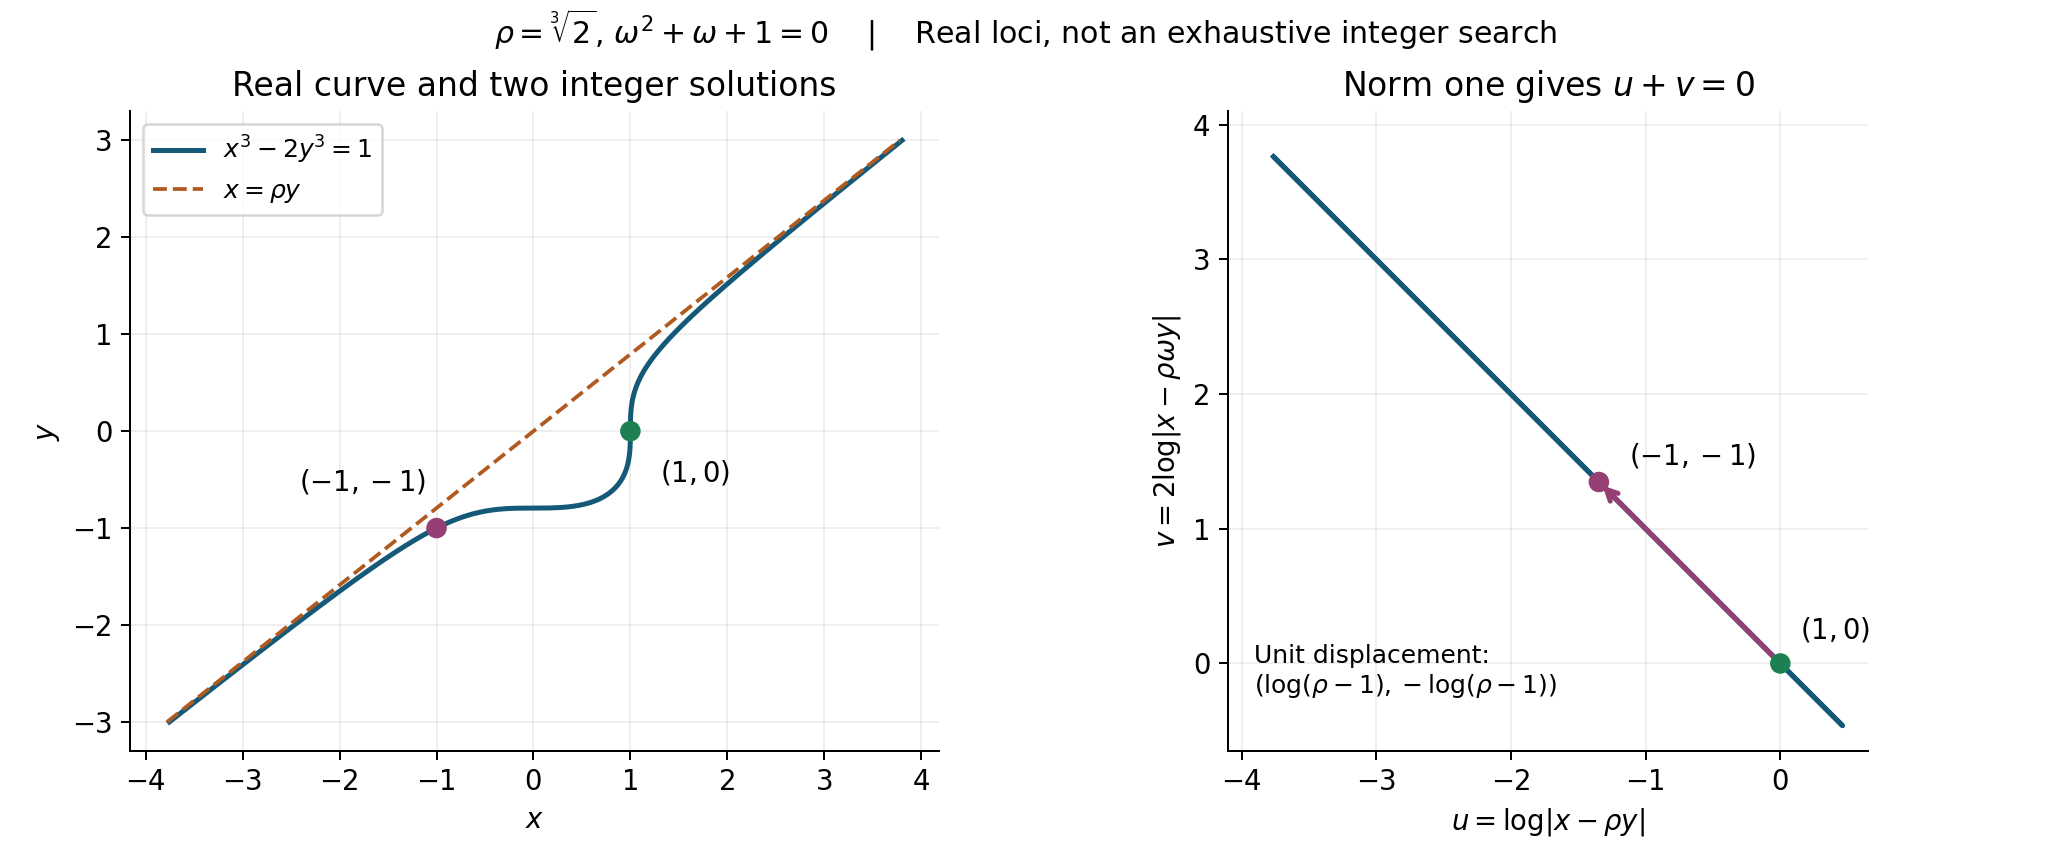
\includegraphics[keepaspectratio,alt={The real cubic and its logarithmic norm coordinates}]{../figures/thue-factor-geometry.png}}
\par\smallskip
\begin{flushleft}\small
\emph{Figure 13.1.}
\end{flushleft}
\end{minipage}\par\medskip
 Left: the real curve \(x^3-2y^3=1\), its line
\(x=\rho y\), and the two displayed integer solutions. Right: the same
real points under \((x,y)\mapsto(\log|x-\rho y|,
2\log|x-\rho\omega y|)\). Equation (13.41) puts them on the line
\(u+v=0\). The two marked solutions are separated by the logarithm
vector of the unit \(\rho-1\). The curves depict real points and do not
assert an enumeration of integer solutions.

The bound \(2^{N_0}\) makes exhaustive search finite. It is much too
large for direct computation. A complete resolution needs a proved
reduction of that bound and a certificate covering the remaining cases;
Lesson 21 develops those procedures. The two substitutions above alone
do not prove completeness.

\subsection{7. Exercises}\label{exercises}

\textbf{1. (Easy: the three-factor relation.)} For
\(\beta_j=x-\theta_jy\), verify \[
(\theta_1-\theta_2)\beta_3+
(\theta_2-\theta_3)\beta_1+
(\theta_3-\theta_1)\beta_2=0.
\] Then derive the two coefficients in (13.12), keeping their signs.

\textbf{2. (Medium: why three distinct factors matter.)} Construct
infinitely many integer solutions of \(x^2-2y^2=1\), and explain why no
bound depending only on the height of its fixed right-hand side can
hold. Also give a degree-three form with only two distinct factors over
a suitable number field for which the same failure occurs.

\textbf{3. (Medium: a relative cubic equation.)} Apply Theorem 13.2 to
\(x^3-2y^3=m\), first for \(x,y\in O_{\mathbb Q(\rho)}\) and
\(m\in\mathbb Q(\rho)^\times\), and then for rational integers. State
explicit bounds in the real embedding using (13.37).

\textbf{4. (Hard: an effective irrationality exponent.)} Starting from
the integer bound for a general irreducible integral binary form, prove
(13.19) for every rational \(p/q\), including errors greater than one.
Express the resulting \(\tau(\rho)\) through the two-logarithm route of
Lesson 12.

\textbf{5. (Medium: the unknown exponent.)} Explain where the normalized
coefficient \(B'\) is essential in Theorem 13.5. Check all cases in
which a logarithm is zero, or the two original terms have opposite
signs.

\textbf{6. (Hard: a coefficient-free family.)} Verify the rational-base
choices, nonvanishing and radius conditions in the proof of Theorem
13.6. Explain why replacing the large radius by \(E=2\) for all \(b\)
would not give the same coefficient-free argument.

\subsection{8. Solutions}\label{solutions}

\textbf{1.} The coefficient of \(x\) is
\(\theta_1-\theta_2+\theta_2-\theta_3+\theta_3-\theta_1=0\). The
negative of the coefficient of \(y\) is \[
\theta_3(\theta_1-\theta_2)+
\theta_1(\theta_2-\theta_3)+
\theta_2(\theta_3-\theta_1)=0
\] by cancellation of its six products. Multiplication by \(M\) gives
(13.11). Move its first summand to the right and divide by
\((\theta_2-\theta_1)\gamma_3\eta_3\). The right side is \(1\); the left
coefficients and unit ratios are exactly \(\alpha,\beta,u,v\) in
(13.12). Distinctness and nonzero factors justify every division.

\textbf{2.} Expand \[
(3+2\sqrt2)^k=x_k+y_k\sqrt2\qquad(k\ge0).
\tag{13.43}
\] The binomial theorem makes both coefficients integers. Taking the
conjugate product gives \(x_k^2-2y_k^2=1\). They are infinitely many
distinct pairs, since \(3+2\sqrt2>1\) and its positive powers are
distinct. More explicitly \[
x_{k+1}=3x_k+4y_k,\qquad y_{k+1}=2x_k+3y_k,
\] starting from \((1,0)\), so the positive coordinates grow. Their
heights are unbounded while \(h(1)=0\). For a degree-three
counterexample over number fields, take \(K=\mathbb Q(\sqrt2)\) and
\(F(X,Y)=X^2Y\). With the unit \(\epsilon=3+2\sqrt2\), the pairs
\((x,y)=(\epsilon^k,\epsilon^{-2k})\in O_K^2\) all satisfy \(F(x,y)=1\)
and have unbounded height. Equivalently, the monic-in-\(X\) form
\(X^2(X-Y)\) admits \((x,y)=(\epsilon^k,\epsilon^k-\epsilon^{-2k})\).
This example separates the three-distinct-root condition from a degree
count.

\textbf{3.} Work in the splitting field \(L=\mathbb Q(\rho,\omega)\).
The calculations (13.34)--(13.37) give \(C=N_0/2\). For
\(x,y\in O_{\mathbb Q(\rho)}\), Theorem 13.2 yields \[
\max\{h(x),h(y)\}\le\frac{N_0}{2}\max\{h(m),1\}.
\tag{13.44}
\] The height inequality at any embedding \(\sigma\) of this
degree-three field is \(|\sigma z|\le e^{3h(z)}\). Thus \[
\max\{|\sigma x|,|\sigma y|\}
\le\exp\!\left(\frac{3N_0}{2}\max\{h(m),1\}\right).
\tag{13.45}
\] For rational integer \(m\ne0\) this is at most \((2|m|)^{3N_0}\). If
\(x,y\) are also rational integers, their own height formula removes the
embedding factor \(3\), giving the sharper \((2|m|)^{N_0}\) in (13.38).

\textbf{4.} Let \(F\) be the homogenized primitive minimal polynomial of
\(\theta\), and let \(C_{\mathbb Z}\ge1\) satisfy (13.18). For every
\(q\ge1\), \(F(p,q)\ne0\); otherwise \(p/q\) would be a rational root.
The bound on \(q\) gives \(|F(p,q)|\ge q^{1/C_{\mathbb Z}}/2\). When
\(|\theta-p/q|\le1\), each other factor has modulus at most
\(1+|\theta-\theta_j|\), so (13.21) follows. Division gives \(c=1/(2A)\)
and \(\tau=1/C_{\mathbb Z}\). For a larger error, \(c q^{-n+\tau}\le1\),
giving the same claim directly. No reduced-fraction assumption was
needed. For \(\rho\), use \[
\tau(\rho)=\frac1{54(2T_0+G(6+2T_0))+160},\qquad
T_0=5+2V,
\tag{13.46}
\] with \(V,G\) explicitly defined in (13.37); \(c=1/50\). Here \(G\) is
supplied by the complete many-to-two reduction and unit-equation proof,
ultimately using Theorem 7.1. Thus the displayed value traces back to
the proved two-logarithm constant \(21600\), not to an unspecified
effective constant.

\textbf{5.} The term \(B'=1/a_2+n/H\) becomes at most \(1+n/H\), whereas
the main height product is at most \(2H\log X\). After comparison with
the upper estimate and division by \(H\log X\), only \(t=n/H\) remains
in (13.28). If \(Y=X\), then \(\log(Y/X)=0\), but \(\Gamma\ne0\) because
\(c\ne0\). If \(A=B\), the other logarithm is zero; the same
nonvanishing remains. Both cannot be zero in the difference case.
Theorem 7.1 permits these bases equal to one. Opposite original signs
give a sum of positive terms, bounded above by \(|c|\), so no
logarithmic estimate is needed. The small-denominator case
\(|c|\ge P/2\) is (13.24). These alternatives cover every sign and size
possibility.

\textbf{6.} A nontrivial positive solution has \(y\ge b+2\), as the
first paragraph of Theorem 13.6 proves. For \(b\ge5\), the four integers
\((y,x,b+1,b)\) satisfy all hypotheses of Corollary 7.7, and its radius
is \(E=b\). The quotient \(1/\eta=\log(b+1)/\log b<5/4\) is bounded
independently of \(b\). This is precisely the cancellation of
coefficient size used in (13.31). For \(b\le4\), the
prime-exponent-vector argument rules out dependence;
\(a_1=\log y>1,\ 1\le a_2\le2\) meet the height cutoffs, and \(E=2\)
meets both radius inequalities. The form equals \(\log(1+\delta)>0\), so
it cannot vanish. For arbitrary \(b\), a fixed \(E=2\) would leave the
unbounded factor \(a_2\asymp\log b\) in (13.32). The growing radius for
\(b\ge5\) is what removes that factor.

\subsection{Reproducible checks and
references}\label{reproducible-checks-and-references}

The \href{verification/cubic-bounds-check.py}{exact cubic
calculations} verify the trace determinant, the constant substitutions
and the two displayed solutions. The
\href{verification/binomial-check.py}{binomial checks} verify
rational numerical margins and finite sign cases. The proofs above
establish the full ranges; the finite checks are supplementary. The
\href{figure_sources/thue-factor-geometry.py}{figure program}
reproduces Figure 13.1.

\begin{itemize}
\tightlist
\item
  Yann Bugeaud and Kálmán Győry, \emph{Bounds for the solutions of unit
  equations}, Acta Arithmetica 74 (1996), 67--80, Lemma 2.
  \href{https://matwbn.icm.edu.pl/ksiazki/aa/aa74/aa7416.pdf}{Free
  journal PDF}.
\item
  Maurice Mignotte, \emph{A note on the equation \(ax^n-by^n=c\)}, Acta
  Arithmetica 75 (1996), 287--295, Theorems 1--3.
  \href{https://www.impan.pl/shop/en/publication/transaction/download/product/109013}{Free
  journal edition}.
\item
  Yann Bugeaud, \emph{Linear forms in the logarithms of algebraic
  numbers close to 1 and applications to Diophantine equations}, author
  version, Section 3.
  \href{https://irma.math.unistra.fr/~bugeaud/travaux/ConfMumbaidef.pdf}{Freely
  accessible text}.
\item
  Michael A. Bennett, \emph{Rational approximation to algebraic numbers
  of small height: the Diophantine equation \(|ax^n-by^n|=1\)}, Journal
  für die reine und angewandte Mathematik 535 (2001), 1--49, Theorem 1.1
  (orientation statement only).
  \href{https://personal.math.ubc.ca/~bennett/B-Crelle2.pdf}{Free
  author-hosted edition}.
\end{itemize}

\end{document}
